\documentclass[sigconf,anonymous,review]{acmart}

\usepackage{graphicx}
\usepackage{amsmath}
\usepackage{booktabs}
\usepackage{xcolor}

\providecommand{\EvidencePending}[1]{\textcolor{orange}{[EVIDENCE PENDING: #1]}}
\providecommand{\ExpFigTODO}[1]{\textcolor{red}{[EXP/FIG TODO: #1]}}

\settopmatter{printacmref=false}
\renewcommand\footnotetextcopyrightpermission[1]{}

\title{Recursive Sparse-Latent Grammars for Training-Free 3D Generative Growth}

\author{Anonymous Author(s)}
\affiliation{%
  \institution{Anonymous Institution}
  \city{}
  \country{}
}
\email{}

\begin{document}

\begin{abstract}
% Previous abstract variants kept for revision trace:
% Procedural grammars can generate recursive trees, roots, corals, ornaments, and fractal structures, but their outputs often lack the geometry and material plausibility expected from modern 3D assets. Conversely, image-to-3D and native 3D generative models produce visually rich one-shot objects but provide little direct control over multi-depth recursive growth. We explore a training-free bridge between these regimes. Our method represents a recursive asset as a sparse 3D latent state derived from mesh-to-O-Voxel encoding, applies grammar operators directly to sparse support and features, and uses a frozen Trellis2 model as a mesh-derived visual prior for geometry and appearance. A projection operator based on connected-component pruning and re-encoding stabilizes error accumulation across recursive depth. Experiments show that per-depth projection improves mesh connectedness compared with final-only cleanup, supports depth-5 vine/root growth, and extends to branching, porous, ornamental, architectural, and hard-surface transform-copy programs. Trellis2 texture postprocessing is technically compatible with selected projected meshes, but current material quality is category-dependent; we therefore evaluate texture export separately from geometric recursion quality.
% Native 3D generators increasingly expose sparse latent representations that appear well suited for recursive structure: trees, roots, corals, ornaments, and architectural motifs can in principle be grown by repeatedly editing local 3D tokens. In practice, direct use of such generators is unstable. Two-dimensional scaffolds can be ignored or inflated into sheets, direct sparse edits create floating fragments, global flow repair can wash out the intended topology, and final-only cleanup cannot prevent fragments from becoming growth roots at the next recursion depth. We introduce a generation-model-native recursive language over sparse 3D latents. A program state consists of active sparse tokens, their latent features, and grammar-readable anchors. Rule templates propose local growth, frontier accretion, or transform-copy edits, while a frozen Trellis2 model is used for masked local naturalization, decoding, re-encoding, and selected texture export. The key execution principle is projection inside the recursive transition: after each depth, the decoded asset is projected to a connected, admissible state and re-encoded before further rules can fire. This turns connected support into a recursive invariant rather than a post-hoc mesh cleanup target. Experiments on branching, frontier-growth, and transform-copy programs show that per-depth projection stabilizes finite-depth recursive growth, exposes a stability-expression tradeoff across rule families, and supports textured GLB export for selected projected meshes without training a new 3D generator.
Recursive 3D structures such as branching plants, roots, corals, crystals, ornaments, and architectural motifs are naturally described by multi-depth programs, yet modern 3D generators are usually trained as single-scale, single-resolution, one-shot object synthesizers. We introduce a generation-model-native recursive grammar that executes over sparse 3D latent states rather than over 2D scaffolds or terminal meshes. The grammar owns the recursive topology: active sparse support, latent features, typed handles, attachment certificates, rule traces, and finite-depth scheduling. A frozen Trellis2-style generator supplies the native sparse representation, masked local realization, decoding, and re-encoding; selected projected meshes can also be exported through its texture/PBR path. Projection is the execution semantics that keeps the recursive state admissible: after each depth, the decoded asset is projected to a connected, reusable state and re-encoded before later rules can fire. Current evidence shows that this per-depth projection stabilizes conservative finite-depth growth relative to direct sparse editing and final-only cleanup, while aggressive fork, radial, and DLA-like operators expose the present stability-expression boundary. \EvidencePending{Fill final quantitative improvement numbers after the matched baseline matrix is complete.}
\end{abstract}

\maketitle

\section{Introduction}

% Previous introduction opening kept for revision trace:
% Recursive structures are central to many natural and stylized 3D assets. Trees branch across scale, roots and vines compete for free space, corals and crystals accrete at exposed frontiers, and architectural ornaments repeat motifs through local transformations. Classical procedural modeling gives explicit control over these phenomena through L-systems, iterated function systems, diffusion-limited aggregation, and space-colonization algorithms~\cite{lindenmayer1968lsystemsI,prusinkiewicz1990abop,barnsley1988fractalsEverywhere,runions2007spacecolonization,witten1981dla,sander2000dlaReview}. These systems are controllable and interpretable, but their outputs are usually scaffolds: curves, tubes, voxel clusters, or hand-designed meshes whose local surface quality and material detail fall short of modern generated assets.
% Large 3D generative models offer the complementary capability. Recent image-to-3D and native 3D asset generators can synthesize detailed geometry and appearance from a single image or text-conditioned image prior~\cite{shapE2023,trellis2024,trellis2project,assetgen2024,dreamgaussian2023,hunyuan3d2025}. TRELLIS and TRELLIS.2 are especially relevant because they represent assets with sparse structured 3D latents that can be encoded from meshes and decoded back into geometry and material latents. However, these models are designed primarily for one-shot generation or localized editing, not for repeatedly applying a formal recursive program while preserving an evolving scaffold.
% Our experiments indicate that naive bridges fail. Rendering a recursive program as a 2D point or line drawing and feeding it to image-conditioned 3D generation produces out-of-distribution sheets and fragments. Conversely, globally resampling or repairing the latent state with the flow model often overwrites the recursive topology. These failures suggest that the generator should not own the whole object. Instead, the recursive program should own the support and attachment structure, while the frozen generator should contribute local shape and appearance priors only where the program introduces new growth.
% We therefore ask: can a frozen native 3D generator be used as the state space and local prior of a recursive grammar? We propose a \emph{recursive sparse-latent grammar} (R-SLG). Starting from a mesh root, we encode the asset into Trellis2's sparse O-Voxel/SLAT state, apply grammar operators directly to sparse coordinates and features, decode the result to a mesh, and insert a projection step before the next recursive depth. This projection is not post-hoc cleanup: it is part of the recursive map and prevents small disconnected errors from becoming new growth roots. The resulting pipeline supports finite-depth recursive assets in which procedural rules control structure and the generator supplies mesh-derived visual priors. Our current emphasis is therefore not infinite scene generation or unconstrained semantic editing, but a narrower and testable problem: how to make repeated recursive edits stable in a frozen sparse 3D generative representation.

% Replaced introduction body kept for revision trace:
% Sparse latent 3D generators suggest a direct route to recursive modeling. Instead of asking a model to synthesize a complete object in one shot, one could grow a tree, root, coral, ornament, or architectural asset by repeatedly editing only the currently active 3D tokens. This would make the generator's native state space the substrate of a recursive program: topology would be controlled by rules, while local geometry and appearance would be supplied by a learned asset prior.
% The direct version of this idea fails for a specific reason. Native 3D generators are strong local and object-level priors, but they are not recursive execution engines. When a procedural scaffold is rendered as a 2D condition, image-to-3D generation often produces sheets, blobs, or disconnected fragments instead of preserving the intended branching topology. When sparse coordinates are edited directly, small floating components accumulate across depth. When a global flow sampler is used as a repair step, it can replace the grammar's topology with the generator's preferred object-level shape. When cleanup is deferred until the final mesh, invalid fragments may already have acted as parents, frontiers, cached motifs, or material sources in intermediate states.
% These failures point to a different formulation. The generator should not own the global recursive structure. Instead, the recursive program should own the sparse support, anchors, and attachment graph, and the frozen generator should act as a masked local prior around rule-proposed edits. We therefore formulate recursive asset synthesis as a \emph{generation-model-native recursive language over sparse 3D latents}. The language executes over the same kind of sparse state used by the 3D generator, but its semantics are grammar-first: rules select handles, propose local token edits, preserve attachment certificates, and project each decoded asset back to an admissible connected state before the next depth.
% This framing differs from both classical procedural modeling and one-shot 3D generation. Classical grammars expose recursion and control through L-systems, iterated function systems, diffusion-limited aggregation, and space-colonization algorithms~\cite{lindenmayer1968lsystemsI,prusinkiewicz1990abop,barnsley1988fractalsEverywhere,runions2007spacecolonization,witten1981dla,sander2000dlaReview}, but they typically output curves, tubes, voxels, or hand-designed meshes that require substantial surface and material authoring. Modern 3D generators synthesize detailed assets from image or text-conditioned priors~\cite{shapE2023,trellis2024,trellis2project,assetgen2024,dreamgaussian2023,hunyuan3d2025}, but they provide no native guarantee that a multi-depth recursive program remains attached, addressable, and editable. Our goal is narrower and more testable than unbounded world generation: finite-depth recursive assets whose structure is controlled by a sparse-latent grammar and whose local realization is supported by a frozen 3D generator.

Recursive algorithms are a basic language for 3D structure. They explain how trees branch across scale, roots and vines compete for space, corals and porous aggregates accrete at exposed frontiers, crystals and ornaments repeat local motifs, and architectural elements split, extrude, and recur. Classical graphics systems already encode these ideas through L-systems, iterated function systems, diffusion-limited aggregation, space-colonization growth, and shape grammars~\cite{lindenmayer1968lsystemsI,prusinkiewicz1990abop,barnsley1988fractalsEverywhere,witten1981dla,sander2000dlaReview,runions2007spacecolonization,stiny1972shapegrammars,mueller2006procedural}. They remain valuable because their recursive structure is explicit, controllable, and inspectable. Their limitation is not a lack of structure, but the cost of turning symbolic or geometric scaffolds into assets with plausible local surfaces, materials, and export-ready detail.

Modern 3D generators provide the complementary asset prior, but their training objective is usually object-level synthesis rather than recursive execution. Set-latent and end-to-end object-latent models such as 3DShape2VecSet and Shap-E learn compact object priors and can generate rich shapes from global or conditional latent codes~\cite{shape2vecset2023,shapE2023}. These representations are powerful object generators, but their intermediate states are not necessarily designed for repeated rule-level addressing, local caching, transform-copy, or per-depth attachment checks. Sparse structured latent generators, including TRELLIS and TRELLIS.2, expose a more operational substrate: sparse token support, latent features, mesh-to-sparse encoding, sparse-to-mesh decoding, masked local sampling, and a texture/PBR export path~\cite{trellis2024,trellis2project}. This makes sparse latents a plausible entry point for recursive 3D programs. \EvidencePending{Add a controlled experiment comparing sparse-latent recursion against set-latent/end-to-end object-latent or mesh-only alternatives.}

The naive entry point still fails. Rendering a recursive program as a 2D point or line scaffold and passing it to image-to-3D generation can inflate branches into sheets, blobs, or fragments. Editing sparse coordinates directly creates small floating components that can become parents, frontiers, cached motifs, or material sources at later depths. A global flow or diffusion repair step can make a local region look plausible while washing out the grammar topology. Final-only cleanup is too late because invalid intermediate handles may already have fired. \EvidencePending{Complete diagnostic failure panels for 2D scaffold entry, direct sparse editing, global repair, and final-only cleanup under the same root/depth protocol.}

These failures motivate a generation-model-native recursive grammar rather than a procedural scaffold followed by generator cleanup. The grammar owns the recursive support, typed handles, local transforms, attachment certificates, rule traces, and projection schedule. Rule templates emit sparse local proposals; the frozen generator supplies masked local realization, decoding, and re-encoding; projection defines the execution semantics that returns each decoded asset to an admissible connected state before the next recursion depth. Texture and PBR are treated as selected export capabilities for projected meshes, not as evidence for topology or as a core contribution.

Our target is therefore finite-depth recursive asset synthesis, not universal procedural modeling, physical growth simulation, or unbounded world generation. We study whether sparse-latent recursive states can remain attached, addressable, and reusable under repeated rule execution, and whether selected projected states can be exported through a frozen 3D generator's asset path.

\paragraph{Contributions.}
This paper makes the following contributions:
\begin{itemize}
  \item We introduce a generation-model-native recursive language over sparse 3D latents, where programs operate on sparse token support, latent features, and grammar-readable anchors rather than on 2D scaffolds or post-hoc meshes.
  \item We define compact rule-template semantics for recursive growth, frontier accretion, transform-copy, and local refinement over sparse latent states.
  \item We introduce projection-stabilized execution, including model-native admissibility checks, connected projection, and recursive state re-encoding, to prevent invalid fragments from becoming later growth handles.
  \item We evaluate finite-depth recursive assets across branching, frontier-growth, and transform-copy families under separated structural, mesh-diagnostic, and export protocols. \EvidencePending{Fill final quantitative claims: matched baselines, root/tip metrics, and improvement numbers.}
\end{itemize}
Selected projected meshes can be exported through the frozen Trellis2 texture/PBR route; we treat this as an asset-readiness capability rather than a structural contribution.

\begin{figure*}[t]
  \centering
  \includegraphics[width=\textwidth]{figures/teaser_candidate_layout_v3_20260509.png}
  \caption{Mesh-based teaser for recursive generative growth. The main result panels use Trellis2 textured GLB renders from selected projected recursive meshes. The bottom strip uses programmatic PBR material on mesh renders only to expose local zoom-in geometry, and is not a Trellis2 texture result. The radial and DLA panels illustrate breadth and boundary cases rather than uniform final-asset quality.}
  \label{fig:teaser}
\end{figure*}

\section{Related Work}

\subsection{Procedural and Recursive Modeling}
% Previous related-work paragraph kept for revision trace:
% Procedural modeling provides the formal substrate for recursive geometry. L-systems and related grammar systems describe branching form through symbolic rewriting~\cite{lindenmayer1968lsystemsI,prusinkiewicz1990abop}, while iterated function systems formalize transform-copy self-similarity~\cite{barnsley1988fractalsEverywhere}. Space-colonization models generate tree structures by competing growth tips against spatial attractors~\cite{runions2007spacecolonization}. Diffusion-limited aggregation produces branching clusters and porous accretion patterns through local stochastic attachment~\cite{witten1981dla,sander2000dlaReview}. These approaches are valuable because they expose explicit structure, but they do not by themselves provide the local surface plausibility and material richness expected from generated 3D assets. We use them as structural baselines and reinterpret several of their operations as sparse latent grammar operators.
Procedural modeling is the closest historical substrate for recursive geometry. L-systems describe plant-like branching through parallel symbol rewriting and turtle interpretation~\cite{lindenmayer1968lsystemsI,prusinkiewicz1990abop}. Iterated function systems formalize transform-copy self-similarity~\cite{barnsley1988fractalsEverywhere}. Diffusion-limited aggregation and related frontier processes generate branching clusters and porous accretion by local stochastic attachment~\cite{witten1981dla,sander2000dlaReview}. Space-colonization models grow trees from competing tips and attractors~\cite{runions2007spacecolonization}. Shape grammars and CGA-style rules split, extrude, replace, and repeat architectural or ornamental elements~\cite{stiny1972shapegrammars,mueller2006procedural}. We do not position these systems as weak baselines. They provide strong structural control, and we use them as restricted domains of the same recursive-language view. The gap we target is different: how to execute analogous recursive programs inside the native sparse state of a frozen 3D generator while preserving asset-level local realization.

\subsection{3D Generative Models and Sparse Latent Representations}
% Previous 3D-generation paragraph kept for revision trace:
% 3D generation has shifted from explicit hand-designed priors toward learned asset distributions. Large datasets such as Objaverse and Objaverse-XL enable broad object-level training~\cite{objaverse2023,objaverseXL2023}, while text/image-conditioned generators such as Shap-E, DreamGaussian, Meta 3D AssetGen, Hunyuan3D, and TRELLIS synthesize geometry or textured meshes from high-level prompts or images~\cite{shapE2023,dreamgaussian2023,assetgen2024,hunyuan3d2025,trellis2024}. TRELLIS.2 targets higher-quality PBR 3D asset generation and supports image-conditioned generation through a native 3D pipeline~\cite{trellis2project}. Our work is not a new generator; it repurposes the sparse representation exposed by a frozen generator as the state of a recursive program. This differs from one-shot asset generation because the same state is repeatedly modified, projected, and re-encoded across depth.
Large 3D datasets such as Objaverse and Objaverse-XL have enabled learned object priors at asset scale~\cite{objaverse2023,objaverseXL2023}. Current systems span implicit representations, Gaussian assets, mesh-producing pipelines, compact object latents, and sparse structured latents. Set-latent or object-latent models such as 3DShape2VecSet and Shap-E learn strong whole-object priors~\cite{shape2vecset2023,shapE2023}, while image- or text-conditioned systems such as DreamGaussian, Meta 3D AssetGen, Hunyuan3D, TRELLIS, and TRELLIS.2 synthesize meshes or textured assets from high-level conditions~\cite{dreamgaussian2023,assetgen2024,hunyuan3d2025,trellis2024,trellis2project}. These systems are effective one-shot generators, but a global object latent is usually not an execution state with explicit recursive handles, attachment certificates, cached motifs, transform-copy support, and rule traces. Sparse structured latent models are more relevant to our setting because they expose sparse token support, token features, mesh-to-sparse encoding, sparse-to-mesh decoding, masked local updates, and selected material/PBR export. Our work is not a new generator; it asks whether this exposed sparse representation can be used as the state space of a recursive grammar. \EvidencePending{Add direct empirical comparison to end-to-end object-latent or mesh-only alternatives.}

\subsection{Generative Control, Editing, and Evaluation}
Training-free editing methods show that frozen generative models can be reused without retraining. In 2D diffusion and flow models, SDEdit- and FlowEdit-style procedures modify images by partially resampling a noisy trajectory~\cite{sdeedit2021,flowedit2024}; analogous ideas appear in mask-based image editing and recent native 3D latent or structured-field editing systems~\cite{nano3d2025,voxhammer2025,latte3d2025,inpaintslat2025}. Structure-conditioned 3D systems add skeletons, point priors, or inpainting networks to improve controllability~\cite{skadapter2026,pointsTo3D2026}. These methods are important because they show that local control and frozen priors can coexist, but they usually perform a single semantic edit, completion, or structure-conditioned generation. We require repeated, grammar-driven, stateful recursive execution: a local edit must leave valid handles, frontiers, and attachment state for later derivation steps.

Evaluating such assets also requires metrics beyond object-level image quality. We track connected components, largest-component ratio, root reachability, orphan mass, depth stability, branch or frontier preservation, and renderability; for branching and porous cases we draw on quantitative morphology descriptors used for reconstructed trees and voxelized porous structures~\cite{raumonen2013treeModels,martinez2018minkowskiPorosity}. We use fractal descriptors cautiously because branching objects are not always strictly self-similar under simple box-counting estimators~\cite{cheeseman2022fractalCaution}. \EvidencePending{Complete root/branch/tip semantic metrics, mesh validity metrics, latent stability metrics, seed statistics, and mean/std reporting for the matched baseline matrix.}

\section{Preliminaries}

\subsection{Recursive Asset Generation}
We use ``recursive generation'' in the standard grammar sense: a finite state is repeatedly rewritten by rules, and a geometric interpretation maps the resulting derivation to an asset. L-systems use parallel symbol rewriting followed by turtle interpretation, iterated function systems repeatedly apply contractive transforms, and shape grammars rewrite local shape parts under contextual rules~\cite{lindenmayer1968lsystemsI,prusinkiewicz1990abop,barnsley1988fractalsEverywhere,stiny1972shapegrammars,mueller2006procedural}. For this paper, a recursive asset program consists of an initial state $s_0$, a rule library $\mathcal R$, a scheduler that selects rules at derivation depth $d$, and an interpretation map that produces geometry. A finite-depth generated asset is
\[
s_{d+1}=\operatorname{Rewrite}(s_d,\mathcal R_d,\xi_d),
\qquad
x_D=\operatorname{Interp}(s_D),
\quad d=0,\ldots,D-1.
\]
This definition is intentionally modest: it covers symbolic derivations, transform-copy systems, frontier growth, and shape-grammar style replacement without claiming infinite recursion or physical simulation. Our method will replace the abstract state $s_d$ with a sparse generator-native state augmented by recursive handles and anchors. \EvidencePending{Tighten this definition after checking graph-grammar and shape-grammar derivation terminology.}

\subsection{Sparse Generator State}
Let $\theta$ denote a frozen sparse structured 3D generator. We write its native state as
\[
z=(V,F),
\]
where $V\subset h\mathbb Z^3$ is sparse token support and $F:V\rightarrow\mathbb R^q$ stores token features. A condition $y$ may be an image, text-derived guide, category hint, material guide, or empty condition. The generator exposes a mesh-to-sparse encoder $\operatorname{Enc}_{\theta}$, a sparse-to-mesh decoder $\operatorname{Dec}_{\theta}$, and a local masked sampler or naturalizer $\mathcal N_{\theta}$:
\[
z=\operatorname{Enc}_{\theta}(x,y),\qquad
x=\operatorname{Dec}_{\theta}(z,y),\qquad
z'=\mathcal N_{\theta}(z;m,y,\xi).
\]
For TRELLIS/TRELLIS.2-style systems, the useful middleware is not merely final mesh generation; it is the exposed sparse support, latent features, codec, possible masked/local update path, and selected texture/PBR export route~\cite{trellis2024,trellis2project}. When a projected mesh $x^\star$ is stable enough for asset inspection, we write optional export as
\[
g=\operatorname{Tex}_{\theta}(x^\star,y_m),
\]
where $g$ is a textured GLB/PBR asset and $y_m$ is an optional material guide. This texture path is an export capability of the frozen generator, not the structural mechanism of the recursive grammar. \ExpFigTODO{User needs to provide sparse voxel / Trellis-style generator pipeline figure: image/mesh condition -> sparse support/features -> decoder -> mesh/PBR asset.}

\section{Method}

% 中文写作纲要：Method 的主线是 formal grammar system，而不是 root mesh -> Trellis2 -> cleanup 的工程流水线。顺序：problem/state/grammar/central operator/classical limits/masked prior/projection/cache and finite-depth limits.
\begin{figure*}[t]
  \centering
  % Previous overview preserved for comparison: figures/method_system_grammar_polished_20260508.pdf
  \includegraphics[width=\textwidth]{figures/method_system_ps_rslg_v3_20260509.pdf}
  \caption{Overview of Projection-Stabilized Recursive Sparse-Latent Grammar. A typed grammar controls symbols, anchors, transforms, and sparse support proposals. Trellis2 supplies the mesh-derived sparse state, masked local sampler, decoder, re-encoder, and optional material export. Projection is inside the recursive transition: each step selects an admissible model-native recursive state and re-encodes before the next grammar rule.}
  \label{fig:method-overview}
\end{figure*}

\subsection{Problem Setting}
We formulate recursive 3D asset synthesis as execution of a grammar program over the native sparse state of a frozen 3D generator. Let $x_0$ be a root mesh or generated root asset, let $z_0=\operatorname{Enc}_{\theta}(x_0,y)$ be its sparse state, let $y$ be an optional image, text, category, or material condition, and let $D$ be a finite recursion depth. The method defines recursive handles over $z_d$, uses rule templates to propose local edits, invokes the frozen generator only for masked local realization, and applies model-native projection before the next derivation step:
\[
z_{d+1}=
\operatorname{Enc}_{\theta}\!\left(
\Pi_{\theta,\lambda_d}\!\left(
\operatorname{Dec}_{\theta}
\left(
\mathcal T_{\theta}(z_d;\mathcal R_d,y,\xi_d)
\right)
\right)
\right),
\quad
x_D=\operatorname{Dec}_{\theta}(z_D,y).
\]
Here $\mathcal R_d\subseteq\mathcal R$ is the selected rule set, $\xi_d$ includes rule choice, frontier sampling, local generative sampling, or sample selection, and $\Pi_{\theta,\lambda_d}$ is an admissibility-constrained state-selection operator. We call the resulting formalism a \emph{Projection-Stabilized Recursive Sparse-Latent Grammar} (PS-RSLG).

The grammar owns global recursive structure: typed handles, transforms, attachment, frontiers, constraints, projection parameters, and caches. The frozen generator is not asked to invent or repair topology after the fact. It supplies the sparse native representation, masked local shape/material priors, decoding, re-encoding, and optional asset export.

\subsection{Core State and Handles}
% Previous 3.2 state definition kept for revision trace:
% At depth $d$, PS-SLG maintains $S_d=(C_d,F_d,U_d,A_d,B_d,M_d,H_d,K_d)$. Here $C_d\subset \{0\}\times h\mathbb{Z}^3$ is the active O-Voxel/SLAT-style sparse support with budget $|C_d|\leq T_{\max}(d)$. The feature map $F_d:C_d\rightarrow\mathbb{R}^{q_s}\times\mathbb{R}^{q_m}\times\mathbb{R}^{q_a}$ stores shape features, optional texture or PBR features, and auxiliary grammar attributes such as age, branch radius, semantic type, local frame code, ownership, and confidence. $U_d$ is a typed symbol string or graph, with symbols $u_i=(\sigma_i,\ell_i,T_i,\Omega_i,\alpha_i,\nu_i)$. $A_d$ stores occupancy, attractors, frontiers, component and attachment graphs, collision regions, quality estimates, and symmetry or lattice metadata. $B_d$ stores edit masks, blend kernels, boundary regions, and hard clamps. $M_d$ stores material intent, texture latent state, PBR parameters, material masks, and export metadata. $H_d$ records depth, seeds, rule traces, transform traces, projection parameters, and diagnostics. $K_d$ stores motif, latent, transform, LOD, visible-window, sampler, and material caches.
We write the recursive state at depth $d$ as the minimal sparse-latent object
\begin{equation}
z_d=(\mathcal V_d,\mathbf F_d,\mathcal A_d).
\end{equation}
Here $\mathcal V_d\subset h\mathbb Z^3$ is the active sparse token support, $\mathbf F_d:\mathcal V_d\rightarrow\mathbb R^q$ stores the generator-native latent features attached to those tokens, and $\mathcal A_d$ is the grammar-readable anchor structure. The anchors include typed handles, local frames, ownership regions, attachment edges, frontier labels, and optional material handles. A handle is written as
\begin{equation}
h_i=(\sigma_i,T_i,\Omega_i,\alpha_i),
\end{equation}
where $\sigma_i$ is its type, $T_i$ is a local frame, $\Omega_i\subseteq \mathcal V_d$ is its owned support or target region, and $\alpha_i$ stores local attributes such as radius, age, material intent, or rule priority.

This minimal state separates the recursive semantics from implementation bookkeeping. Masks, random seeds, rule traces, diagnostic scores, projection schedules, cached motifs, and texture-export metadata are auxiliary data used by the executor, but they are not the primary mathematical state a reader must remember. The important invariant is that each active handle must be addressable in the sparse support and attached to the recursive scaffold unless it is explicitly marked as an inactive descriptor. Thus a floating component is not merely a visual artifact: if it enters $\mathcal A_d$ as an active handle, it can contaminate all later recursion depths.

We therefore maintain a connected-state domain. Let $\mathcal V_d^{\mathrm{root}}\subset \mathcal V_d$ denote root anchors or scaffold tokens, and let $G_\eta(\mathcal V_d)$ be the $\eta$-neighborhood graph over sparse tokens. The attached support is
\begin{equation}
\mathcal V_{\mathrm{att}}(z_d)=
\{v\in\mathcal V_d:\ v\to \mathcal V_d^{\mathrm{root}}\ \mathrm{in}\ G_\eta(\mathcal V_d)\}.
\end{equation}
We use the violation
\begin{equation}
V_{\mathrm{conn}}(z_d)=
1-\frac{\operatorname{mass}(\mathcal V_{\mathrm{att}}(z_d))}
{\operatorname{mass}(\mathcal V_d)+\epsilon}.
\end{equation}
An admissible recursive state satisfies bounded connectivity, occupancy, renderability, material, and token-budget violations:
\begin{align}
\mathcal Z_{\mathrm{adm}}(\lambda)=
\{z:\;& V_{\mathrm{conn}}(z)\le\epsilon_c,\quad
V_{\mathrm{frontier}}(z)=0,\quad
V_{\mathrm{occ}}(z)\le\epsilon_o,\nonumber\\
& V_{\mathrm{mat}}(z)\le\epsilon_m,\quad
|\mathcal V(z)|\le T_{\max}\}.
\end{align}
The condition $V_{\mathrm{frontier}}(z)=0$ means that every active frontier or growth handle has a valid attachment path to the root scaffold.

\subsection{Rule Templates as a Recursive Language}
% Previous 3.3 grammar tuple kept for revision trace:
% A PS-SLG was written as the tuple $\mathcal{G}=(\Sigma,\mathcal{T},\mathcal{R},\mathcal{I},\mathcal{S},\Pi,\mathcal{N}_{\theta}^{s},\mathcal{N}_{\theta}^{m},\mathcal{D}_{\theta},\mathcal{E}_{\theta},\mathcal{P},\mathcal{C},\mathcal{O},\mathcal{L})$, where the terms represented typed alphabets, transforms, rules, interpretation, scheduling, constraints, frozen naturalization kernels, decoder, encoder, projection, caches, observables, and scoring. Rules had the larger form $r:X(\omega,\Omega,\ell,a,h)\Rightarrow\{(X_j,T_j,\Omega_j,\rho_j,\mu_j,\beta_j,\psi_j,\zeta_j,\tau_j,\pi_j,\kappa_j)\}_{j=1}^{m}$.
The language consists of three objects: typed handles, rule templates, and realization operators. A rule is a local rewrite template over handles,
\begin{equation}
\rho:\ h_i\mapsto
\{(\sigma_j,\tau_j,\Omega_j,m_j,\kappa_j,\pi_j,\eta_j)\}_{j=1}^{k}.
\end{equation}
Each emitted item creates or updates a handle of type $\sigma_j$, local transform $\tau_j$, target or ownership region $\Omega_j$, edit mask $m_j$, feasibility condition $\kappa_j$, proposal kernel $\pi_j$, and optional sampler or material schedule $\eta_j$. The proposal kernel may instantiate frontier growth, branch splitting, stochastic attachment, transform-copy, local refinement, material transport, or cache lookup. Thus the rule is not a mesh macro; it is a small local program that emits projectable sparse support together with the handles needed by the next recursive step.

Rules are executed only when their feasibility conditions hold. In particular, a materialized proposal $\Delta\mathcal V$ must lie in the projectable reachable domain, or the rule must also emit a connector mask whose completed state remains admissible:
\begin{align}
\Delta\mathcal V &\subset
\mathcal R_{\mathrm{proj}}(z_d;b_d,r_d),
\quad\text{or}\nonumber\\
\exists B,F',\mathcal A':\quad
z'&=(\mathcal V_d\cup\Delta\mathcal V\cup B,F',\mathcal A')
\in\mathcal Z_{\mathrm{adm}}(\lambda_d),\quad
\operatorname{cost}(B)\le b_d.
\end{align}
Here $\mathcal R_{\mathrm{proj}}$ contains sparse coordinates that are close enough, collision-free enough, and cheap enough to connect back to the attached scaffold. The connector $B$ is a grammar or model-proposed editable mask that must be naturalized before it becomes active support; it is not a manual mesh bridge. This condition is the semantic difference between recursive growth and unconstrained latent editing: a patch is not active merely because it looks plausible locally; it must remain usable by the next recursive step.

\begin{table*}[t]
  \centering
  \caption{Representative rule families in the sparse-latent recursive language. The table keeps only operators used by the current method narrative and experiments; material export is handled separately as asset compatibility.}
  \label{tab:rule-families}
  \begin{tabular}{@{}p{0.13\textwidth}p{0.42\textwidth}p{0.35\textwidth}@{}}
    \toprule
    Rule family & Definition / proposal & Feasibility role \\
    \midrule
    \textbf{Grow} & Emit $\Delta\mathcal V=\{v+\delta:\ v\in\Omega_i,\ \delta\in\mathcal N_\eta,\ s(v,\delta)>0\}$ from an attached frontier handle. & Accepted tokens must remain root-reachable or carry a connector mask. \\
    \textbf{Branch} & Split one handle $h_i$ into $k$ child handles with frames $T_i\circ\tau_j$ and disjoint target masks $m_j$. & Children inherit parent attachment and must pass collision and occupancy tests. \\
    \textbf{Attach} & Sample frontier cells with probability proportional to a hitting or attraction score, then add the sampled local support. & Used for porous/coral stress tests; proposals are inactive unless attached or model-completed under a mask. \\
    \textbf{Copy} & Transform-copy support and features, $\widehat{\mathcal V}_j=Q_h(\tau_j(\mathcal V_d\cap\Omega_j))$, then merge by masked feature averaging. & Tests latent transform-copy and motif reuse; copied handles must remain projectable. \\
    \textbf{Split/Extrude} & Decompose a local frame into face, tile, portal, or segment handles and emit bounded extrude/repeat support. & Used for architectural and hard-surface motifs; keeps rule scope local. \\
    \textbf{Refine} & Densify terminal or zoom-region handles by allocating additional local support under a fixed token budget. & Currently a planned effective-resolution experiment rather than a final claim. \\
    \bottomrule
  \end{tabular}
\end{table*}

Given a selected rule set $\mathcal R_d$, rule proposal and sparse merge are summarized as
\begin{equation}
\tilde z_{d+1}=\mathcal M(z_d,\operatorname{Prop}_{\mathcal R_d}(z_d)).
\end{equation}
For a transform-copy proposal, the support and features are
\begin{equation}
\widehat{\mathcal V}_j=Q_h(\tau_j(\mathcal V_d\cap\Omega_j)),\qquad
\widehat{\mathbf F}_j(Q_h(\tau_jv))=\mathcal T_j^F\mathbf F_d(v),
\end{equation}
and masked feature merge is
\begin{equation}
\mathbf F^+(v)=
\frac{w_0(v)\mathbf F_d(v)+\sum_j w_j(v)\widehat{\mathbf F}_j(v)}
{w_0(v)+\sum_jw_j(v)+\epsilon},
\qquad
w_j(v)=m_j(v)\beta_j(v).
\end{equation}
Material handles use the same transport-and-merge logic, but are kept distinct from the geometric claim: current evidence supports texture/PBR export for selected projected meshes, while per-depth material naturalization remains an extension of the same semantics.

\subsection{Projection-Stabilized Execution}
% Previous 3.4 operator chain kept for revision trace:
% Let $R_d^\star=\mathcal{S}(S_d,\mathcal{R})$ be the selected rule set. The central recursive transition was written as $S_{d+1}=\mathcal{C}_{d+1}\circ\mathcal{E}_\theta\circ\mathcal{P}_{\lambda_d}\circ\mathcal{D}_\theta\circ\mathcal{N}_{\theta,m}^{\tau_d^m\rightarrow0}\circ\mathcal{N}_{\theta,s}^{\tau_d^s\rightarrow0}\circ\Theta_{\Pi_d}\circ\operatorname{Merge}_{B_d,M_d}\circ\operatorname{Prop}_{R_d^\star}(S_d)$. The useful retained content is that projection is inside the recursive map, and transform-copy merge used $\widehat C_j=Q_h(T_j(C_d\cap\Omega))$ with masked feature averaging.
The recursive transition is intentionally compact:
\begin{equation}
z_{d+1}=
\operatorname{Enc}_{\theta}
\left[
\Pi_{\theta,\lambda_d}
\left(
\operatorname{Dec}_{\theta}
\left(
\mathcal T_{\theta}(z_d;\mathcal R_d,y)
\right)
\right)
\right].
\label{eq:compact-recursive-transition}
\end{equation}
The operator $\mathcal T_{\theta}$ contains rule selection, sparse proposal, masked merge, feasibility filtering, and optional local naturalization. The decoder $\operatorname{Dec}_{\theta}$ maps the sparse state to a mesh or occupancy proxy, $\Pi_{\theta,\lambda_d}$ selects an admissible connected recursive state, and $\operatorname{Enc}_{\theta}$ re-encodes the projected asset before the next depth. Projection is therefore inside the recursive map, not a final cleanup pass.

For clarity, the hidden structure of $\mathcal T_{\theta}$ is
\begin{align}
\mathcal R_d&=\operatorname{SelectRules}(\mathcal A_d,\mathcal R,z_d,\xi_d),\\
\mathcal P_d&=\operatorname{Prop}_{\mathcal R_d}(z_d),\\
\tilde z_{d+1}&=\mathcal M(z_d,\operatorname{Filter}_{\lambda_d}(\mathcal P_d)),\\
\bar z_{d+1}&=\mathcal N_{\theta}(\tilde z_{d+1};m_d,y,\xi_d),
\end{align}
so Eq.~\eqref{eq:compact-recursive-transition} is equivalently
\begin{equation}
z_{d+1}=
\operatorname{Enc}_{\theta}
\!\left[
\Pi_{\theta,\lambda_d}
\!\left(
\operatorname{Dec}_{\theta}(\bar z_{d+1})
\right)
\right].
\end{equation}
The frozen sampler $\mathcal N_{\theta}$ is therefore part of the grammar semantics, but only as a masked stochastic realization operator after rule feasibility has fixed the editable region.

\paragraph{Recursive sparse-latent program execution.}
A transition begins by selecting active handles from $\mathcal A_d$ and choosing rules by type, priority, frontier state, budget, and optional symmetry orbit. The selected rules instantiate sparse proposals, which are rejected or deferred unless they lie in the projectable reachable domain or carry a valid model-completable connector mask. Accepted proposals are merged through their masks and blend kernels, then filtered by occupancy competition and attachment constraints. Edited regions may be locally naturalized by the frozen masked sampler while anchor regions are hard-clamped. The state is then decoded, projected to an admissible connected asset, re-encoded, and returned to the grammar with updated handles, frontiers, material metadata, diagnostics, and caches. Classical systems such as L-systems, IFS, DLA, and space colonization can be viewed as restricted rule families; details are included in the supplementary appendix.

\begin{figure}[t]
  \centering
  \fbox{\begin{minipage}{0.92\columnwidth}
  \small
  \textbf{Algorithm 1: PS-RSLG execution}

  \textbf{Input:} root asset $x_0$, rule library $\mathcal R$, condition $y$, depth $D$, projection schedule $\{\lambda_d\}$.

  \textbf{Output:} projected recursive state $z_D$ and asset $x_D^\star$.
  \begin{enumerate}
    \item Encode $z_0\leftarrow\operatorname{Enc}_\theta(x_0,y)$ and initialize root handles, frontiers, and rule traces.
    \item For $d=0,\ldots,D-1$:
    \begin{enumerate}
      \item Select active handles and rules $\mathcal R_d\leftarrow\operatorname{Select}(\mathcal A_d,\mathcal R,z_d)$.
      \item Instantiate sparse proposals $\mathcal P_d\leftarrow\operatorname{Prop}_{\mathcal R_d}(z_d)$ with masks, transforms, and feasibility certificates.
      \item Reject, defer, or keep proposals using attachment feasibility and token-budget checks.
      \item Merge accepted proposals and apply $\mathcal N_\theta$ only on editable masks while clamping anchor regions.
      \item Decode, select an admissible projected state, and re-encode:
      $x_{d+1}\leftarrow\operatorname{Dec}_\theta(\bar z_{d+1},y)$,
      $x_{d+1}^{\star}\leftarrow\Pi_{\theta,\lambda_d}(x_{d+1},\mathcal A_d)$,
      $z_{d+1}\leftarrow\operatorname{Enc}_\theta(x_{d+1}^{\star},y)$.
      \item Update surviving handles and mark detached descriptors inactive before the next rule selection.
    \end{enumerate}
  \end{enumerate}
  \end{minipage}}
  \caption{Algorithmic semantics of PS-RSLG. The grammar controls support, handles, and feasibility; the frozen generator is restricted to masked naturalization, decoding, re-encoding, and selected material export.}
  \label{alg:ps-rslg-execution}
\end{figure}

\subsection{Masked Local Naturalization}
The frozen generator is used as a local naturalization prior, not as a global repair model. In SDE form,
\begin{equation}
du_t=f_\theta(u_t,t,y)\,dt+g(t)\,dW_t,
\end{equation}
or, for a deterministic flow,
\begin{equation}
\frac{d u_t}{dt}=v_\theta(u_t,t,y).
\end{equation}
The trajectory variable $u_t$ is the sampler state; $z_d$ remains the recursive program state. Let $m_d$ be the sparse edit mask selected by the rule and clipped by connectivity feasibility. A single reverse step is clamped as
\begin{equation}
u_{t-\Delta t}=
(1-m_d)\odot z_{\mathrm{anchor}}
+m_d\odot\Phi_{\theta,t}(u_t,y).
\label{eq:masked-flow-clamp}
\end{equation}
Equivalently, for sparse features on edited tokens,
\begin{equation}
\mathbf f_i'=
(1-\alpha_i)\mathbf f_i^{\mathrm{rule}}
+\alpha_i\mathbf f_i^{\theta},
\qquad i\in m_d.
\end{equation}
The sampler therefore naturalizes local shape or material; it does not decide the global recursive topology.

\subsection{Model-Native Projection}
Projection is an admissibility-constrained state selection step, not a manual mesh-repair stage. After decoding a candidate asset, the executor decides which decoded support can remain active recursive state before the next rule selection. Detached components are converted to inactive descriptors or deleted before re-encoding; they are not allowed to become parents, frontiers, or cached motifs. Optional connectors are admitted only when a grammar rule proposes an editable connector mask and the frozen generator naturalizes that mask before it is re-encoded as active support.

We express the projection as
\begin{equation}
\Pi_{\theta,\lambda_d}(x,\mathcal A_d)
=
\operatorname*{arg\,min}_{x'\in\mathcal X_{\mathrm{adm}}(\lambda_d)}
d_{\theta}(x,x')+
\lambda_{\mathrm{state}}V_{\mathrm{frontier}}(x',\mathcal A_d)
\lambda_{\mathrm{inactive}}M_{\mathrm{orphan}}(x',\mathcal A_d),
\end{equation}
where $\mathcal X_{\mathrm{adm}}(\lambda_d)$ denotes decoded assets whose re-encoded state satisfies $\mathcal Z_{\mathrm{adm}}(\lambda_d)$, $d_{\theta}$ is a model-space or codec-space discrepancy, $V_{\mathrm{frontier}}$ penalizes active handles without a root path, and $M_{\mathrm{orphan}}$ measures support that would survive only as detached descriptors. In the current implementation this is approximated by a conservative prune-only active-state policy: only root-attached decoded support and certified model-completed connector regions are re-encoded as active state. Post-hoc traditional mesh repair, if used for diagnostics, is a baseline rather than the proposed projection operator.

\ExpFigTODO{Run projection variants: no projection, final-only, per-depth prune-only, model-proposed bridge, and traditional repair baseline. Report deletion mass, pruned component count, orphan handles, active-handle survival, branch/tip preservation, topology drift, and LCR.}
\ExpFigTODO{User needs to provide/approve a projection mechanism figure: invalid orphan tokens become inactive vs model-proposed connector under mask vs re-encoded admissible state.}
\EvidencePending{Need projection variants proving the main operator is model-native state selection rather than manual patching.}

\paragraph{Why final-only cleanup is insufficient.}
Let $e(z)$ combine connectivity, orphan-frontier, renderability, and material violations. If each projection satisfies
\begin{equation}
e(\Pi_{\theta,\lambda_d}(x,\mathcal A_d))\le\epsilon_P
\end{equation}
and the decode/re-encode round trip adds at most $\epsilon_E$, then the executed recursive states obey
\begin{equation}
e(z_d)\le \epsilon_P+\epsilon_E,\qquad d=1,\ldots,D.
\end{equation}
Final-only cleanup lacks this invariant because an invalid component can be selected as a parent, copied as a motif, sampled as a local condition, or stored in a cache before the final mesh is cleaned. This is the central reason to place projection inside Eq.~\eqref{eq:compact-recursive-transition}.

% Previous post-3.5 sparse-competition and projection-stability text kept for revision trace:
% \subsection{Sparse Competition and Masked Naturalization}
% For a proposed action $a$ at coordinate $c$, PS-SLG used a generic sparse competition score
% \[
% \begin{aligned}
% \psi(a,c;S_d)=
% {}&\lambda_{\mathrm{att}}\phi_{\mathrm{att}}
% -\lambda_{\mathrm{occ}}\phi_{\mathrm{occ}}
% -\lambda_{\mathrm{col}}\phi_{\mathrm{collision}}
% +\lambda_{\mathrm{front}}\phi_{\mathrm{frontier}}
% {}\\
% &+\lambda_{\mathrm{grp}}\phi_{\mathrm{orbit}}
% +\epsilon_{\theta}(a,c,\xi).
% \end{aligned}
% \]
% The frozen sampler was then restated in SDE/flow form, with a masked clamp
% \(Z_{t-\Delta t}\leftarrow(1-\mu_\Omega)\odot Z_{\mathrm{anchor}}+\mu_\Omega\odot\Phi_{\theta,t}(Z_t,y)\)
% and feature blending \(F'(c)=(1-\alpha_d(c))F^+(c)+\alpha_d(c)F_\theta(c)\).
% \subsection{Projection-Stabilized Recursion}
% The old duplicate projection section defined \(\mathcal{S}_{\mathrm{adm}}(\lambda)=\{S:V_k(S)\leq\epsilon_k,\ |C(S)|\leq T_{\max}\}\),
% \(V_{\mathrm{frag}}(S)=1-\operatorname{mass}(C_{\mathrm{largest\ attached}})/(\operatorname{mass}(C)+\epsilon)\),
% an ideal \(P_\lambda(S)\), and the invariant \(e(S_d)\leq\epsilon_P+\epsilon_E\).
% This material is now folded into the earlier projection paragraph using the current state notation
% \(z_d=(\mathcal V_d,\mathbf F_d,\mathcal A_d)\) and the recursive transition in Eq.~\eqref{eq:compact-recursive-transition}.

\subsection{Operator Scheduling and Sparse Competition}
For a proposed action $a$ at sparse token $v\in\mathcal V_d$, PS-RSLG uses a conservative competition score only for operators whose candidates compete for the same local support:
\[
\begin{aligned}
\psi(a,v;z_d)=
{}&\lambda_{\mathrm{att}}\phi_{\mathrm{att}}
-\lambda_{\mathrm{occ}}\phi_{\mathrm{occ}}
-\lambda_{\mathrm{col}}\phi_{\mathrm{collision}}
+\lambda_{\mathrm{front}}\phi_{\mathrm{frontier}}
{}\\
&+\lambda_{\mathrm{grp}}\phi_{\mathrm{orbit}}
+\epsilon_{\theta}(a,v,\xi).
\end{aligned}
\]
The attachment term $\phi_{\mathrm{att}}$ is the negative sparse-graph distance from the candidate to $\mathcal V_{\mathrm{att}}(z_d)$, saturated at the local rule radius. The occupancy term $\phi_{\mathrm{occ}}$ counts already-owned tokens in the candidate mask. The collision term $\phi_{\mathrm{collision}}$ penalizes overlap with forbidden regions or incompatible handle ownership. The frontier term $\phi_{\mathrm{frontier}}$ rewards candidates that extend an active frontier direction or hit an attractor assigned to that handle. The orbit term $\phi_{\mathrm{orbit}}$ is used only for symmetry or lattice programs and scores consistency with other scheduled orbit members. The generator preference $\epsilon_{\theta}$ is optional and weak in the current experiments; it can rank locally plausible feature samples but cannot override attachment feasibility. \ExpFigTODO{Add operator scheduling / sparse competition figure and run corresponding case examples with active handles, candidate frontier tokens, rejected collision tokens, accepted attached proposal, and next handles.}

\subsection{Recursive Refinement Scope}
One-shot Trellis2 generation is bounded by a fixed latent grid, decoder budget, and object-level sampling pass. A recursive sparse-latent program instead spends its token budget locally: at depth $d$, only handles in $\mathcal A_d$ whose masks intersect active frontier, terminal detail, or transform-copy regions emit new support. This is a hypothesis about effective addressable detail, not yet a measured resolution claim. If each active handle emits at most $k_d$ accepted tokens and projection keeps the realized state within budget, then
\[
|\mathcal V_{d+1}|
\leq
\min\{T_{\max}(d+1),\ |\mathcal V_d|+\sum_{h_i\in\mathcal H_d}k_i\}.
\]
The claim is therefore not that the method outputs an infinite mesh or already exceeds the generator's native resolution. The current paper studies finite-depth projected assets and selected multi-scale views. Stronger effective-resolution claims require dedicated metrics such as terminal handle count per unit volume, minimum generated feature scale, local token density, detail survival after decode/project/re-encode, and comparison to one-shot generation under matched budgets. \ExpFigTODO{Major experiment needed: recursive effective resolution with depth, local detail metrics, multi-level naturalization, and one-shot generator comparison.}

\subsection{Material Handles and Trellis2 Texture Export}
Material is represented as grammar metadata attached to anchors, masks, and exported components, not as evidence for structural correctness. A material handle stores a local intent label, guide condition, PBR-channel availability, and ownership region. Transform-copy rules transport material handles with the same local frame as geometry; grow and branch rules inherit or blend parent handles across their masks; projection removes material handles whose geometry is pruned and marks uncertain seams for export validation. When a projected mesh $x_d^\star$ is stable enough for asset inspection, the frozen Trellis2 texture/PBR path can be called as
\[
g_d=\operatorname{Tex}_{\theta}(x_d^\star,y_m),
\]
where $g_d$ is a GLB/PBR asset and $y_m$ is an optional image, category, or material guide.

This separation is important for evaluation. Geometry recursion and material recursion have different failure modes: a textured GLB can import and render successfully while the underlying mesh still has holes, thin sheets, or face-level fragmentation. Conversely, a neutral mesh may be structurally useful before the material path is polished. We therefore treat Trellis2 texture export as an asset-readiness claim for selected projected meshes, and not as proof of recursive connectivity, DLA physics, or crystal growth correctness.

Texture export also inherits the effective-resolution semantics above. The recursive program may allocate additional sparse support only around active handles, but Trellis2 textured mesh export is called on a finite projected mesh $x_d^\star$, so PBR channels, UVs, and GLB packaging are evaluated at the realized depth rather than over an infinite logical program. This lets selected assets show high local detail or repeated motifs without claiming that material generation itself is recursively consistent across unexpanded cache descriptors.

\subsection{Scope, Complexity, and Export}
The present paper claims finite-depth recursive asset generation with $D<\infty$ and $|\mathcal V_d|\leq T_{\max}(d)$. Each depth pays for rule selection, sparse proposal and merge, optional masked naturalization, decoding, projection, and re-encoding. This makes the cost higher than a single one-shot generator pass, but it provides intermediate states that can be inspected, projected, and reused by later rules. Runtime and memory should therefore be reported per depth, not only for final export. \ExpFigTODO{Measure runtime, GPU memory, per-depth encode/decode/projection cost, token growth, mesh growth, and texture export cost.}

Texture/PBR export is separated from structural recursion. The texture path is called only on selected projected meshes, and GLB/PBR diagnostics support asset-readiness rather than topology. Symmetry closure, cache descriptors, visible-window logical recursion, and detailed classical-system reductions are treated as supplementary material or future extensions unless they are directly supported by the main experiments.

\section{Experiments and Results}

\paragraph{Claims under test.}
The experiments are organized around two current claims. First, a connected recursive sparse-latent grammar with projection inside the transition stabilizes conservative finite-depth recursive growth relative to direct sparse editing or final-only cleanup. Second, once a mesh has passed the projection and renderability checks, the frozen Trellis2 texture/PBR path can export selected recursive meshes as inspectable GLB assets. We do not claim that every operator family is solved, that smoke-test exports are final-quality assets, or that DLA/crystal-inspired examples reproduce physical growth processes. \EvidencePending{Complete same-root tree/root/vine matched matrix before turning relative-stability language into final quantitative claims.}

\begin{table*}[t]
  \centering
  \caption{Claim map for the current paper draft. The table is used to keep the main narrative conservative: topology, mesh diagnostics, and material export are deliberately separated.}
  \label{tab:claim-map-current}
  \begin{tabular}{@{}p{0.20\textwidth}p{0.31\textwidth}p{0.25\textwidth}p{0.17\textwidth}@{}}
    \toprule
    Claim & Main evidence & Required protocol & Must not claim \\
    \midrule
    Sparse-latent recursive language & state, handles, rule templates, classical reductions & formal semantics and algorithm boxes & arbitrary universal procedural language \\
    Sparse substrate over object latents & Trellis/Trellis2 operations expose addressable support, codec, masked sampling, and export & controlled comparison to set-latent, object-latent, or mesh-only alternatives \EvidencePending{Run or cite controlled comparison} & sparse latents are always superior \\
    Per-depth projection stabilizes recursion & direct vs final-only vs per-depth ablations & components, LCR, root reachability, orphan mass & all operators become clean meshes \\
    Classical systems are restricted domains & IFS, L-system, space-colonization, DLA/frontier, shape-grammar reductions & equations and fair baseline table & visual dominance over mature procedural systems \\
    Non-tree scaffold families are possible & coral/DLA-inspired and crystal/lattice-like connected scaffolds & occupancy or surface-voxel connectivity plus mesh renders & physical DLA, physical crystallization, watertight topology \\
    Trellis2 texture/PBR export is compatible with selected projected meshes & textured GLB renders for selected vine, coral, crystal, and baseline assets & GLB import/render, PBR availability, surface-voxel diagnostic & texture as connectivity proof \\
    Branch semantics remain usable & root-attached handles, branch/tip preservation, junction zooms & root reachability, orphan-tip rate, endpoint and path-to-root metrics \EvidencePending{Complete semantic branching metrics} & connected occupancy equals full tree topology \\
    Depth and parameter rows show method behavior & same-condition depth and density rows with zoom panels & fixed guide, camera, renderer, and texture schedule & calibrated monotonic control unless measured \\
    \bottomrule
  \end{tabular}
\end{table*}

\paragraph{Main paper, figures-only pages, and supplement boundary.}
The main text must stand on the figures and tables cited here; it does not rely on appendix figure or table numbers. Claim-bearing figures are the projection ablation, matched structural baseline matrix, selected connected vine/root, coral, and crystal scaffold rows, and the texture/export QA table. Broad guide sweeps, full result matrices, cache/LOD probes, bismuth guide sensitivity, and extra depth galleries should be moved to figures-only pages only when they contain figure/caption material, or otherwise to the supplement. Hard-DLA bridge repair, fragmented fork/radial/echo variants, blocky cache-selected outputs, partial transfers, and uninspected GLBs are diagnostic or boundary cases rather than main positive evidence. \ExpFigTODO{Before submission, split current gallery-heavy figure set into main claim figures, at most two figures-only pages, and supplemental diagnostics.}
\ExpFigTODO{Re-render all visual results on pure white background with standard paper-style subfigure layout, no in-image labels beyond subfigure letters, consistent camera/framing, and no presentation-style panels.}

\subsection{Tasks}
We evaluate three task families chosen to stress different parts of the language: tree, root, and bush branching for connected handle recursion; coral, crystal, and porous frontier growth for attachment and surface-fragmentation stress tests; and transform-copy assets for recursive motifs, portals, and local zoom structure. The non-tree tasks are included as controlled scaffold and stress-test evidence unless their mesh and render diagnostics pass the same protocol as the branching assets.

\subsection{Baselines}
Baselines include pure procedural meshes, smoothed/remeshed procedural meshes, one-shot Trellis2 image-to-3D, image-entry then recursion, direct coordinate grammar, full flow repair, masked flow repair, weak masked blend, final-only projection, projection-stabilized masked blend, and attachment-aware grammar variants. Procedural baselines are used for structural control and fair mesh-render comparison; they are not treated as material-quality upper bounds.
\ExpFigTODO{Run fair baselines including mesh-space recursion, one-shot Trellis2, direct sparse edit, global repair, masked repair, final-only projection, and ours.}
\ExpFigTODO{Critical experiment: prove sparse-latent grammar operations outperform mesh-space procedural postprocessing and ordinary Trellis texture export.}
\ExpFigTODO{Naturalization ablation required: rule-only, no-N, masked-N, global-N, weak blend, with/without projection.}
\ExpFigTODO{Run root-quality and seed-variation experiments; report success rates and mean/std.}

\subsection{Metrics}
We report mesh validity and renderability, connected-component statistics, largest-component ratio, depth stability, branch/tip preservation, token growth, texture-latent compatibility, and visual contact sheets from consistent mesh renders. For connectivity, the primary structural metric is a voxel-occupancy 6-neighborhood proxy rather than raw face connectivity, because procedural tube baselines may export adjacent branch segments without shared vertices. Raw face components, tolerance-based vertex welding, non-manifold diagnostics, and render success are retained as mesh-quality diagnostics. For textured GLB exports we additionally use a surface-sampled voxel connectivity diagnostic, which is less sensitive to UV/material seams than raw face graphs while still exposing visible small-component fragments. Texture/PBR metrics report GLB export, Blender import, channel availability, and render warnings; they support asset-readiness, not topology.
\ExpFigTODO{Literature search and implement metrics: mesh validity, skeleton topology, morphology, latent stability, effective resolution, material diagnostics.}
\ExpFigTODO{Re-evaluate texture export as compatibility only; report GLB/PBR diagnostics separately from geometry metrics.}

We report every result under a protocol-separation rule. Structural recursion is evaluated by occupancy or surface-voxel connectedness, root reachability, orphan mass, and branch/frontier proxies. Mesh quality is evaluated separately through raw face components, non-manifold warnings, weld/remesh status, Blender import, and renderability. Texture/PBR export is evaluated by GLB size, material guide, channel availability, render success, and seam warnings. Same-condition depth or parameter rows are labeled as method-behavior visualizations unless they change exactly one algorithmic design choice under a matched ablation protocol. This separation directly prevents textured renders from substituting for topology evidence.

\begin{figure*}[t]
  \centering
  \includegraphics[width=\textwidth]{figures/claim_aligned_metric_summary_20260509.png}
  \caption{Claim-aligned metric summary for the current draft. Occupancy connectedness is the primary structural proxy, while raw mesh or face components are reported as caveats rather than hidden. The right panel reports root-reachability proxies only for families where explicit skeleton or root-handle evidence exists. Red crosses mark DLA bridge-ablation variants that remain negative or partial results despite some improved diagnostics.}
  \label{fig:claim-aligned-metrics}
\end{figure*}

\begin{figure}[t]
  \centering
  \includegraphics[width=\columnwidth]{figures/surface_voxel_connectivity_metric_20260509.pdf}
  \caption{Surface-sampled voxel connectivity diagnostic for selected textured GLB exports. Pyrite and bismuth remain one strict surface-voxel component through depth; the porous case exposes small strict radius-0 fragments but becomes one component under a radius-1 seam/alias-tolerant check. This figure is a renderability diagnostic and does not replace watertight mesh topology tests.}
  \label{fig:surface-voxel-connectivity}
\end{figure}

\paragraph{Current evidence organization.}

% Previous status-report style result narrative kept for revision trace:
% The main result supports the connected-recursion claim. Procedural 2D scaffolds are poor image conditions for Trellis2, mesh-first encoding better preserves recursive geometry, and full flow repair causes topology drift. Per-depth projection is the strongest stabilizer in the current implementation: in the vine depth-5 competition run, the raw decoded mesh contains hundreds of disconnected components, while projection keeps the main recursive support and re-encodes it for the next depth. This evidence is strongest for conservative competition-style branching and weaker for aggressive fork, radial, and echo operators.
% The second result concerns projection-stabilized textureable assets. Texture/export validation succeeds for several projected recursive meshes, producing GLB assets for vine depth-5, tree depth-3, tree portal, DLA competition, and fork-side vine variants. These exports show that projected recursive meshes can enter the Trellis2 texture/PBR path, but the resulting renders remain category-dependent and can expose holes, thin-sheet artifacts, or material mismatch.

\subsection{Per-Depth Projection Stabilizes Conservative Recursive Programs}
The strongest empirical claim is not that all grammars become clean assets, but that projection inside the recursive transition stabilizes conservative recursive programs. Figure~\ref{fig:projection-depth-curves} shows that competition-style sparse growth preserves a dominant component through repeated decode/project/re-encode steps for vine and tree assets. Figure~\ref{fig:space-competition-depth-curves} reports the corresponding token-growth curves: conservative competition grows slowly, while fork and side-branch variants consume more support and enter the current stability-expression boundary.

Table~\ref{tab:projection-ablation} and Figure~\ref{fig:projection-ablation-mesh} give the matched ablation. Direct recursion leaves fragments available throughout execution. Final-only projection removes many fragments from the terminal mesh, but it cannot prevent those fragments from influencing intermediate handles, frontiers, caches, or material state. Per-depth projection is the only tested setting that makes connected support a recursive invariant. In the cleanest vine case, raw mesh components drop from 2059 under direct recursion to one after per-depth projection; in the tree case they drop from 3201 to two. These numbers are raw mesh diagnostics; occupancy-primary connectedness is reported separately when comparing mixed OBJ and GLB sources.

\subsection{Baselines Separate Structural Control from Asset Readiness}
Traditional L-system and space-colonization baselines are structurally strong and should not be treated as strawmen. Figure~\ref{fig:space-colonization-baseline} renders generated OBJ tube meshes with the same Blender protocol used for our method. The baselines expose branch, tip, and coverage structure clearly, but remain schematic and untextured. The matched structural matrix in Table~\ref{tab:matched-structural-baseline-matrix} is therefore a fairness check: under a same-root, same-seed, same-depth, same-renderer protocol, classical baselines and our connected scaffold proxy can all produce root-attached occupancy-connected supports.

The distinction appears when structural supports are passed through a texture/PBR path. Figure~\ref{fig:traditional-texture-baseline} uses the same Trellis2 texture export route for space-colonization, L-system, and DLA-like procedural supports. The latest rerun shows a fairer and stronger baseline than our earlier matched-guide diagnostic: several traditional supports become renderable and near-connected under the surface-voxel proxy, while the DLA-like cluster remains visually blocky. This supports the paper's formulation without treating classical baselines as strawmen: geometry, recursive support, semantic organization, and appearance export must be evaluated separately.

\subsection{Selected Projected Meshes Support Texture and PBR Export}
Projection-stabilized meshes can enter the frozen Trellis2 texture path. Figure~\ref{fig:vine-depth-textured} and Figure~\ref{fig:vine-stage5-guide-sweep} show true Trellis2 textured GLB exports for a vine/root program under fixed or varied public guides, including a depth-5 projected mesh. Figure~\ref{fig:connected-best-expansion-textured}, Figure~\ref{fig:pyrite-hq-depth-textured}, Figure~\ref{fig:crystal-stage4-guide-sweep}, and Figure~\ref{fig:coral-depth-textured} extend the evidence to non-tree connected scaffolds. The strongest current crystal/symmetry example is a pyrite-like lattice program; bismuth remains a guide-sensitivity and stepped-scaffold diagnostic rather than the main non-tree positive case. These figures support texture/PBR compatibility for selected projected meshes, not a claim that all exported GLB face graphs are topology-clean or that material recursion is solved.

\subsection{Depth and Parameter Control Are Method-Behavior Evidence}
Same-condition displays are used to show how the method behaves under depth or parameter changes, not to prove causal ablations. Figure~\ref{fig:vine-zoom} gives a multi-scale mesh render of one recursive vine asset. Figure~\ref{fig:depth-parameter-main-candidate} and Figure~\ref{fig:depth-parameter-mesh-showcase-zoom} show fixed-family depth and parameter rows with zoom crops. Figure~\ref{fig:coral-density-extreme} strengthens the previous weak parameter sweep by using a wider density endpoint range under a fixed guide, renderer, and camera. It demonstrates qualitative controllability of local branching density while retaining occupancy-primary connected support, but it should not be read as a calibrated monotonic law.

\subsection{Current Boundaries}
Figure~\ref{fig:claim-aligned-metrics} summarizes the metric boundary: connected voxel support is the current defensible structural claim, while raw GLB face components are a separate export diagnostic. Figure~\ref{fig:dla-bridge-smoke-rerun} gives a concrete DLA boundary case: post-hoc sparse bridging can improve face-level diagnostics while leaving occupancy support fragmented or worse, whereas a grammar-native volumetric-DLA scaffold is occupancy-connected before such repair. Figure~\ref{fig:result-matrix} is retained as a qualitative breadth overview rather than as a main evidence figure. Aggressive fork, radial, echo, DLA, and post-hoc bridge variants remain useful diagnostics because they explain why projection, attachment feasibility, and grammar-native connected support are necessary; they are not presented as solved final-asset cases.

Current figure placement follows the same rule. Projection ablations, connected vine/root depth rows, the fair traditional texture baseline diagnostic, and the strongest connected coral/crystal scaffold rows belong in the main evidence chain. Broad guide sweeps, result matrices, bismuth guide sensitivity, cache/LOD probes, and extra depth galleries are supplementary unless distilled to one claim-specific panel. Hard-DLA post-hoc bridge, fragmented radial/echo/fork variants, and blocky cache-selected cases are boundary diagnostics. Matplotlib point-cloud previews, partial transfers, and uninspected GLBs are not evidence figures.

\begin{figure}[t]
  \centering
  \includegraphics[width=\columnwidth]{figures/projection_depth_curves_20260508.pdf}
  \caption{Projection-stabilized recursion measured by largest connected component ratio across recursive stages. Stable operators preserve one dominant asset across depth, while aggressive transform/echo operators expose the current stability-expression boundary.}
  \label{fig:projection-depth-curves}
\end{figure}

\begin{figure*}[t]
  \centering
  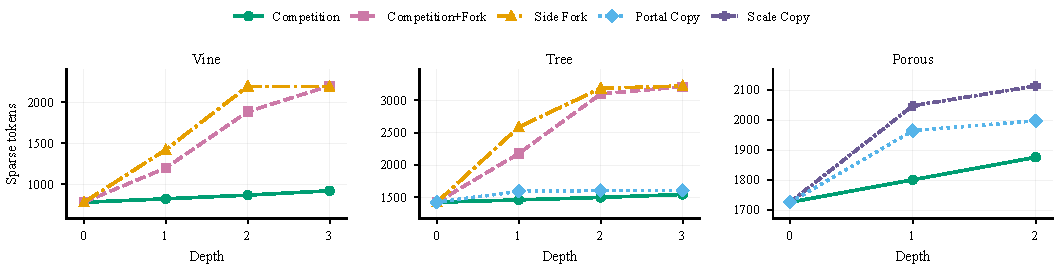
\includegraphics[width=\textwidth]{figures/space_competition_depth_curves_tokens_20260508.pdf}
  \caption{Sparse-token growth curves for current recursive operators. Conservative occupancy competition grows slowly and is therefore the strongest stability baseline; fork and side-branch variants increase expressive capacity but consume more sparse support; portal and scale-down are more relevant to non-tree recursive/zoom applications.}
  \label{fig:space-competition-depth-curves}
\end{figure*}

\begin{figure*}[t]
  \centering
  \includegraphics[width=\textwidth]{figures/space_colonization_blender_contact_sheet.png}
  \caption{Traditional space-colonization baseline rendered from generated OBJ tube meshes with a fixed Blender/Cycles protocol. The baseline is structurally useful for branch/tip/coverage metrics but visually schematic and untextured, providing a fair contrast to mesh-first sparse generative recursion and selected Trellis2 textured GLB exports.}
  \label{fig:space-colonization-baseline}
\end{figure*}

\begin{figure*}[t]
  \centering
  \includegraphics[width=\textwidth]{figures/traditional_baseline_texture_rerun1554_20260509.pdf}
  \caption{Traditional procedural baselines passed through the same Trellis2 texture/PBR export path used for selected PS-RSLG scaffolds. This latest rerun is intentionally a strong and fair baseline: space-colonization and L-system supports become renderable textured GLBs and are near-connected or connected under the surface-voxel proxy, while the DLA-like cluster remains visually blocky. The result supports protocol separation rather than a strawman comparison: texture transfer is possible for classical supports, but recursive scaffold semantics and asset readiness still require separate visual and structural evaluation.}
  \label{fig:traditional-texture-baseline}
\end{figure*}

\iffalse
\begin{figure*}[t]
  \centering
  \includegraphics[width=\textwidth]{figures/traditional_baseline_texture_matched_guide_20260509.png}
  \caption{Matched-guide version of the traditional baseline texture diagnostic. All four baselines use the same vine material guide and Trellis2 texture schedule, so the remaining differences primarily reflect procedural support geometry. The IFS baseline is the strongest in largest-component ratio but is still not single-component under the occupancy proxy.}
  \label{fig:traditional-matched-texture-baseline}
\end{figure*}
\fi

\begin{figure*}[t]
  \centering
  \includegraphics[width=\textwidth,height=0.82\textheight,keepaspectratio]{figures/result_matrix_mesh_20260509.png}
  \caption{Mesh-render result matrix with explicit protocol separation. Green panels are true Trellis2 textured GLB renders; blue panels are fixed programmatic PBR renders used for cleaner material visualization; gray panels are neutral shaded mesh renders used for geometry and operator breadth. No point-cloud previews are used. This matrix is therefore a qualitative status overview, not a claim that every shown result is a successful textured Trellis2 asset.}
  \label{fig:result-matrix}
\end{figure*}

\begin{figure*}[t]
  \centering
  \includegraphics[width=\textwidth]{figures/vine_zoom_in_multiscale_20260509.png}
  \caption{Multi-scale Blender render of a recursive vine mesh. The panels show overview, branch-level recursion, and terminal detail on the same generated mesh family. The material is a fixed programmatic PBR render used to expose local geometry; the figure supports zoom-in inspection of recursive structure but does not claim Trellis2 per-depth texture recursion.}
  \label{fig:vine-zoom}
\end{figure*}

\begin{figure*}[t]
  \centering
  \includegraphics[width=\textwidth]{figures/vine_depth_textured_strip_20260509_vizworker.png}
  \caption{Textured mesh depth progression for one vine/root program under the same public guide image and the same Blender render protocol. The four panels are true Trellis2 textured GLB exports from per-depth projected meshes. They visualize a selected textureable recursive asset under fixed appearance guidance; the figure is not a quantitative ablation or a claim that texture quality is uniform across categories.}
  \label{fig:vine-depth-textured}
\end{figure*}

\begin{figure*}[t]
  \centering
  \includegraphics[width=\textwidth]{figures/vine_stage5_guide_sweep_20260509.png}
  \caption{Depth-5 visual/export closure for the vine metric claim. All four panels use the same projected stage-5 vine mesh, the same Trellis2 texture schedule, and the same Blender camera; only the public guide image changes. The occupancy-primary proxy reports one connected component for all variants, but raw GLB face components remain a diagnostic caveat. This is a guide sweep and a selected textured-mesh display, not a method ablation or a clean-topology claim.}
  \label{fig:vine-stage5-guide-sweep}
\end{figure*}

\begin{figure*}[t]
  \centering
  \includegraphics[width=\textwidth]{figures/depth_parameter_main_candidate_20260509.pdf}
  \caption{Same-condition method-behavior cases. Each row changes one control variable while keeping the grammar family, material/image guide, camera, and renderer fixed. The vine and coral rows show recursive depth progression; the coral-density row changes a compactness parameter at a fixed stage. All panels are mesh or textured-mesh Blender renders. This figure is not an ablation study.}
  \label{fig:depth-parameter-main-candidate}
\end{figure*}

\begin{figure*}[t]
  \centering
  \includegraphics[width=\textwidth,height=0.82\textheight,keepaspectratio]{figures/depth_parameter_mesh_showcase_zoom_20260509.pdf}
  \caption{Same-condition method-behavior visualization with zoom crops. The first two rows vary recursion depth for vine/root and connected coral programs; the third row varies a density/compactness parameter at fixed depth. Cameras, material guides, renderer settings, and grammar family are fixed within each row. The zoom insets are included to expose local recursive structure, not to define an ablation; the parameter row is qualitative control evidence and should not be read as a calibrated monotonic response.}
  \label{fig:depth-parameter-mesh-showcase-zoom}
\end{figure*}

\begin{figure*}[t]
  \centering
  % Previous include preserved for revision trace:
  % \includegraphics[width=\textwidth]{figures/connected_best_expansion_texture_rerun1544_20260509.pdf}
  \includegraphics[width=\textwidth]{figures/connected_scaffold_v2_hq_selected_contact_pure_white_rerun2115_20260509.png}
  % Previous caption preserved for revision trace:
  % Connected best-expansion textured GLB results across different connected scaffold families. The pyrite/bismuth lattice is the strongest current non-plant positive case, with strict surface-voxel connectivity of one component and LCR $1.000$. The porous/octopus scaffold is near-connected at strict radius and connected after a one-voxel tolerance, so it is retained as an organic/porous scaffold candidate rather than a physical DLA claim. The root/vine and sci-fi panels show additional connected scaffold families but are not the strongest visual cases.
  \caption{Pure-white no-ground Blender contact sheet for selected connected scaffold families. The panels emphasize mesh silhouette, attachment, and local scaffold readability without textured-material cues, so the figure supports connected-scaffold visual evidence rather than a claim that all families are solved textured GLB assets.}
  \label{fig:connected-best-expansion-textured}
\end{figure*}

\begin{figure*}[t]
  \centering
  \includegraphics[width=\textwidth]{figures/pyrite_hq_depth_textured_showcase_20260509.pdf}
  \caption{Non-tree depth-control visualization on a connected pyrite-like lattice scaffold under a fixed public material guide and fixed Trellis2 texture schedule. The stages remain occupancy-connected and surface-voxel connected while occupied support and local crystal facets increase with depth. This is the current preferred crystal/symmetry visual line; it supports connected scaffold recursion and PBR export for a crystal-inspired asset, not physical pyrite growth simulation or watertight topology.}
  \label{fig:pyrite-hq-depth-textured}
\end{figure*}

\begin{figure*}[t]
  \centering
  \includegraphics[width=\textwidth]{figures/crystal_stage4_guide_sweep_20260509.png}
  \caption{Guide sweep for connected crystal-inspired stage-4 scaffolds. Each pair fixes the geometry and Trellis2 schedule while changing only the material guide. The pyrite/lattice family is the strongest current crystal/symmetry positive case; the bismuth family is retained as stepped-scaffold and guide-sensitivity evidence because its material guide remains less convincing. These are connected scaffold and export-compatibility results, not physical crystal-growth simulations.}
  \label{fig:crystal-stage4-guide-sweep}
\end{figure*}

\begin{figure*}[t]
  \centering
  \includegraphics[width=\textwidth]{figures/coral_depth_textured_showcase_rerun1640_20260509.pdf}
  \caption{Connected coral/DLA-inspired depth-control visualization under a fixed grammar family and fixed public material guide. In the rerun shown here, all four textured GLB stages are single components under the strict surface-voxel diagnostic with LCR $1.000$. The result is therefore a grammar-native connected-scaffold alternative to post-hoc DLA bridge repair, not a claim that the object follows a physical DLA process.}
  \label{fig:coral-depth-textured}
\end{figure*}

\begin{figure*}[t]
  \centering
  \includegraphics[width=\textwidth]{figures/depth_parameter_mesh_showcase_20260509.png}
  \caption{Same-condition depth and guide-control gallery using textured mesh or Blender mesh renders only. Each row locks the generator family, texture path, camera, and background unless the row explicitly studies material guidance. The full gallery is intended as supplementary method-control evidence; the main text should emphasize the vine and coral rows unless later tuning strengthens the weaker rows.}
  \label{fig:depth-parameter-mesh-showcase}
\end{figure*}

\begin{figure*}[t]
  \centering
  \includegraphics[width=\textwidth]{figures/coral_density_extreme_texture_rerun1900_20260509.png}
  \caption{Same-condition density-parameter control for a connected coral scaffold. The grammar family, recursion stage, public material guide, Trellis2 texture schedule, renderer, and camera are fixed; only the density parameter changes. This endpoint sweep is a method-behavior visualization, not an ablation. It shows that a grammar parameter can change local branching density and mesh/token budget while the occupancy-primary support remains connected.}
  \label{fig:coral-density-extreme}
\end{figure*}

\begin{figure*}[t]
  \centering
  \includegraphics[width=\textwidth]{figures/dla_bridge_smoke_stage1_rerun1455_20260509.pdf}
  \caption{DLA connectivity smoke test rendered as meshes. Hard-DLA remains fragmented after raw projection, and sparse bridging improves face-level diagnostics without making the occupancy support reliably connected. A grammar-native volumetric-DLA scaffold is the strongest route in this test: it is one occupancy component before bridge repair. This supports the paper's conservative claim that connected non-tree assets should be generated with attachment-aware rules rather than repaired after fragmentation.}
  \label{fig:dla-bridge-smoke-rerun}
\end{figure*}

\begin{figure*}[t]
  \centering
  % Previous include preserved for revision trace:
  % \includegraphics[width=\textwidth]{figures/projection_ablation_mesh_contact_20260509.png}
  % Pure-white no-ground contact sheet without zooms:
  % \includegraphics[width=\textwidth]{figures/projection_ablation_pure_white_flat_contact_rerun2105_20260509.png}
  \includegraphics[width=\textwidth]{figures/projection_ablation_pure_white_zoom_20260509.pdf}
  % Previous caption preserved for revision trace:
  % Mesh-rendered projection ablation for conservative competition programs. Each row fixes the root family, operator, depth, renderer, and camera. Direct recursion leaves fragments available throughout execution; final-only projection cleans the final mesh once; per-depth projection projects every decoded state before subsequent handles are selected. The figure visualizes the same trend as Table~\ref{tab:projection-ablation} using Blender mesh renders rather than point-cloud or scatter previews.
  \caption{Pure-white no-ground Blender projection ablation for conservative competition programs, with local zoom crops. Each row fixes the root family, operator, depth, renderer, and camera. Direct recursion leaves fragments available throughout execution; final-only projection cleans the final mesh once; per-depth projection projects every decoded state before subsequent handles are selected. The figure visualizes the same trend as Table~\ref{tab:projection-ablation} using mesh renders without texture, shadow, or ground-plane cues.}
  \label{fig:projection-ablation-mesh}
\end{figure*}

\begin{table*}[t]
  \centering
  \caption{Projection ablation on matched roots, operators, and depth. Direct recursion performs no projection until the final mesh. Final-only projection prunes the final direct mesh once. Per-depth projection decodes, projects, and re-encodes after every recursive step. The component counts and LCR in this table are raw mesh face-connectivity diagnostics for the listed OBJ assets, complementary to the occupancy-primary metric used elsewhere. Conservative competition benefits most clearly; expressive fork variants reveal the stability-expression boundary and require stronger attachment or projection policies.}
  \label{tab:projection-ablation}
  \begin{tabular}{lrrrrrrr}
    \toprule
    Case & Direct comps. & Direct LCR & Final kept & Final LCR & Per-depth raw comps. & Per-depth kept & Per-depth LCR \\
    \midrule
    vine compete d3 & 2059 & 0.9049 & 2 & 0.9934 & 819 & 1 & 1.0000 \\
    tree compete d3 & 3201 & 0.9169 & 4 & 0.9842 & 835 & 2 & 0.9949 \\
    vine compete-fork d3 & 11490 & 0.5178 & 11 & 0.6863 & 2581 & 24 & 0.5758 \\
    tree compete-fork d3 & 12166 & 0.5869 & 20 & 0.6937 & 5538 & 53 & 0.6141 \\
    \bottomrule
  \end{tabular}
\end{table*}

\begin{table*}[t]
  \centering
  \caption{Matched structural baseline matrix at the final recursive depth. All methods use the same root anchor, seed, maximum depth, and mesh-render protocol; classical controls use L-system and space-colonization baselines~\cite{lindenmayer1968lsystemsI,prusinkiewicz1990abop,runions2007spacecolonization}.}
  \label{tab:matched-structural-baseline-matrix}
  \begin{tabular}{llrrrrrr}
    \toprule
    Case & Method & Occ. comps. & Occ. LCR & Root ratio & Tips & Branch nodes & Mesh comps. \\
    \midrule
    tree & L-system & 1 & 1.0000 & 1.0000 & 27 & 13 & 1 \\
    tree & Space colonization & 1 & 1.0000 & 1.0000 & 143 & 89 & 9 \\
    tree & Ours & 1 & 1.0000 & 1.0000 & 9 & 4 & 1 \\
    root & L-system & 1 & 1.0000 & 1.0000 & 27 & 13 & 1 \\
    root & Space colonization & 1 & 1.0000 & 1.0000 & 118 & 78 & 9 \\
    root & Ours & 1 & 1.0000 & 1.0000 & 7 & 3 & 1 \\
    vine & L-system & 1 & 1.0000 & 1.0000 & 4 & 3 & 1 \\
    vine & Space colonization & 1 & 1.0000 & 1.0000 & 124 & 68 & 24 \\
    vine & Ours & 1 & 1.0000 & 1.0000 & 6 & 4 & 1 \\
    \bottomrule
  \end{tabular}
\end{table*}


\begin{table*}[t]
  \centering
  \caption{Trellis2 textured GLB export table. Export status is separated from figure-quality judgement: several cases export valid GLBs but remain visually weak because of holes, thin sheets, material mismatch, or camera/UV artifacts. Public-guide rows use externally sourced reference images as appearance guides and are therefore evaluated as texture/PBR compatibility tests, not as standalone method contributions.}
  \label{tab:texture-qa}
  \begin{tabular}{lrrrrl}
    \hline
    Case & Status & GLB MB & Shape tokens & PBR tokens & Evaluation role \\
    \hline
    vine/root compete & ok & 26.81 & 1608 & 526818 & teaser example \\
    tree compete & ok & 27.59 & 3126 & 778755 & matrix/reference \\
    crown portal & ok & 38.48 & 3362 & 1495359 & transform-copy example \\
    scifi translate & ok & 35.87 & 5860 & 1426673 & hard-surface example \\
    snow arch portal & ok & 27.39 & 4757 & 1485294 & architecture example \\
    island city scale-down & ok & 42.34 & 5017 & 1457076 & Escher proxy, needs camera/material tuning \\
    DLA radial & ok & 36.35 & 6301 & 1130891 & boundary case \\
    public-guide vine & ok & 24.70 & 1594 & 516751 & texture/PBR compatibility \\
    public-guide tree/root & ok & 30.36 & 3149 & 765315 & texture/PBR compatibility \\
    public-guide portal/arch & ok & 22.65 & 3154 & 1040417 & public-guide transform-copy \\
    public-guide porous/crystal & ok & 38.69 & 5031 & 2048463 & PBR compatibility \\
    public-guide scifi/gear & ok & 36.08 & 5860 & 1426673 & mechanical color transfer, holed fragments \\
    public-guide snow arch & ok & 27.61 & 4757 & 1485294 & architecture compatibility \\
    % Previous diagnostic row kept out of the visible table: vine/root initial export & failed & 0.00 & 1608 & 526818 & inference-mode bug fixed \\
    \hline
  \end{tabular}
\end{table*}

\section{Discussion and Limitations}

The current method depends on root quality, transform compatibility is empirical rather than guaranteed, and visual quality still varies strongly across operators. Texture export is now technically functional, but material coherence is not yet reliable enough to replace neutral geometry renders for every result. The method should therefore be presented as a training-free recursive asset generation framework for finite-depth assets, not as a universal infinite 3D generator.

\bibliographystyle{ACM-Reference-Format}
\bibliography{references}

\end{document}
